\subsubsection{shell简介}

在windows系统中，我们使用电脑主要是通过图形化界面点击某个图标来启动某个程序；在linux系统中我们更频繁的使用终端和命令行。然而这些都只是我们控制计算机的表象，真正能够控制计算机硬件（CPU、内存、显示器等）的只有操作系统内核（Kernel），图形界面和命令行只是架设在用户和内核之间的一座桥梁。

考虑到安全等原因，用户不能直接接触内核，因此需要另外再开发一个程序，让用户通过使用这个程序来间接地与内核进行交互。该程序的作用就是接收用户的操作（点击图标、输入命令），并进行简单的处理，然后再传递给内核。用户界面和命令行就是这个另外开发的程序，在 Linux下，这个命令行程序叫做 shell 。

\begin{figure}[H]
    \centering
    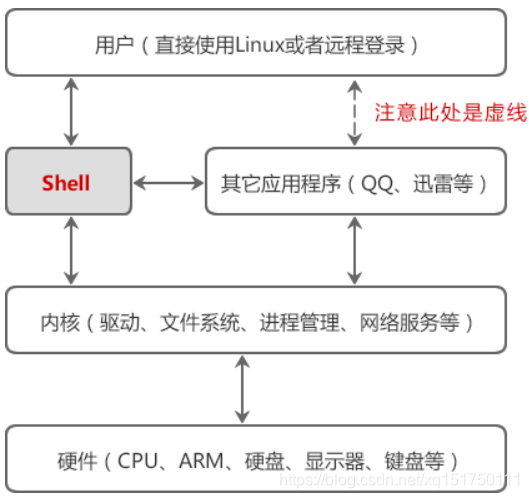
\includegraphics[width=0.7\textwidth]{shell.png}
    \caption{shell工作流程示意图} % 图片标题
    \label{fig:shell} % 图片标签，用于引用
\end{figure}

shell的一大特性就是它是一个应用程序，它连接了用户和 Linux 内核，让用户能够更加高效、安全、低成本地使用 Linux 内核。另一大特性是它是一个命令语言解释器，shell把我们在计算机上的操作或我们的命令，翻译为计算机可识别的二进制命令，传递给内核，以便调用计算机硬件执行相关的操作；计算机执行完命令后，再通过Shell翻译成自然语言，呈现在我们面前。同时，Shell 程序设计语言支持在高级语言里所能见到的绝大多数程序控制结构，比如循环，函数，变量和数组等等。

常见的shell有Bourne shell (sh), C shell (csh), Korn shell (ksh), Bourne Again shell(bash, sh 的扩展), Z shell (zsh), friendly interactive shell (fish) 等等。

启动shell的方法有两种，一是进入linux控制台，二是使用终端（快捷键为ctrl+alt+t）

\subsubsection{简单的shell脚本}

\textbf{新建一个shell脚本}

打开文本编辑器，新建一个文件 test.sh

\begin{tbash}
	vim test.sh
\end{tbash}

然后在shell脚本的第一行输入

\begin{tbash}
	#!/bin/bash
\end{tbash}

\#! 是一个约定的标记，它告诉系统这个脚本需要什么解释器来执行，即使用哪一种 shell。在第一行下面就可以用shell编程语言输入脚本内容了。

\begin{example}
一个最简单的 shell 脚本，运行后打印一行文字：
\begin{tbash}
#!/bin/bash
echo "Hello World !"
\end{tbash}
\end{example}

shell脚本可用于ROS程序自启，即编写一系列命令行操作，启动程序时无需打开终端敲命令行，只需启动一个shell脚本即可。

\textbf{运行shell脚本}

运行shell脚本也有两种方式：

\begin{enumerate}
\item 作为可执行程序

先使脚本具有执行权限

\begin{tbash}
	chmod +x ./test.sh
\end{tbash}

再执行脚本

\begin{tbash}
	./test.sh
\end{tbash}

\item 作为解释器参数

直接运行解释器，其参数就是 shell 脚本的文件名。eg:

\begin{tbash}
	/bin/sh test.sh
	/bin/php test.php
\end{tbash}

这种方式运行的脚本，不需要在第一行指定解释器信息，写了也没用
\end{enumerate}

\begin{exercise}
编写脚本 \texttt{prepare.sh}，依次执行：创建目录 \texttt{mydir}、在其中创建空文件 \texttt{a.txt}、列出 \texttt{mydir} 的内容。分别以"可执行程序"和"解释器参数"两种方式运行该脚本，并观察结果。
\end{exercise}

\subsubsection{linux中的bash}

根据刚刚对shell的介绍可以知道bash也是一种shell，事实上在大多数的linux系统中，bash是默认的缺省shell。当然如果你不想用bash也可以换成其他的shell（比如zsh也很好用）。

bash和shell一样有许多强大的功能，经常用到的有命令补全，通配符，命令历史记录，重定向，管道等等。bash的配置文件分为全局配置文件和个人配置文件：

\begin{center}
\textbf{bash主要文件}
	\begin{tabular}{cc}
		\toprule[1.5pt]
		文件 & 作用\\
		\midrule[1pt]
		$  /etc/profile    $		&系统的主配置文件，用于设置系统范围内的环境变量和其他系统的设置\\
		\texttt{\textasciitilde/.bashrc}		&用于定义用户的命令别名和本地变量\\
		\texttt{\textasciitilde/.bash\_profile}		&用于定义用户的环境变量，运行命令或脚本\\
		\bottomrule[1.5pt]
	\end{tabular}
\end{center}

其中我们会经常对.bashrc文件进行操作。

.bashrc是终端里面指令运行的配置脚本，是系统的隐藏文件，存放在\textasciitilde{} 目录下。.bashrc的功能主要有两个：

\begin{enumerate}
\item 个性化指令alias：alias [指令别名]='原指令'

注意alias和=之间不能有空格

\item 设定环境路径：export PATH=\$PATH:路径
\end{enumerate}

对.bashrc中的内容进行修改后，在下一次打开新终端时修改内容才会生效，或执行source \textasciitilde/.bashrc立刻生效。

\begin{example}
在 \texttt{.bashrc} 中添加一条别名和一个环境路径，让 \texttt{ll} 等价于 \texttt{ls -l}：
\begin{tbash}
alias ll='ls -l'
export PATH=$PATH:/opt/myapp/bin
\end{tbash}
保存后执行 \texttt{source \textasciitilde/.bashrc}，修改立即在当前终端生效。
\end{example}

\begin{exercise}
在你的 \texttt{.bashrc} 中添加别名 \texttt{cls}（等价于 \texttt{clear}），用 \texttt{source} 使其生效并验证；确认无误后将其删除，恢复原状。
\end{exercise}

\subsubsection{linux系统环境变量简介}

linux系统中有非常多的环境变量在控制系统的运行，常用的有：

\begin{enumerate}
\item PATH：决定了shell将到哪些目录中寻找命令或程序

\item HOME：当前用户主目录

\item SHELL：当前用户Shell类型
\end{enumerate}

这里我们主要介绍PATH环境变量

PATH说简单点就是一个字符串变量，当输入命令的时候linux会去查找PATH里面记录的路径，path 配置的路径下的文件可以在任何位置执行，并且可以通过which 可执行文件命令来找到该文件的位置。注意PATH是大写，linux中区分大小写。

我们先来查看一下PATH：

\begin{example}
查看当前的 PATH 环境变量：
\begin{tbash}
echo $PATH
\end{tbash}
\end{example}

终端中会输出

/usr/local/sbin:/usr/local/bin:/usr/sbin:/usr/bin:/sbin:/bin:/usr/games:

/usr/local/games:/usr/lib/wsl/lib:/snap/bin


每个路径中间用:隔开，输入命令时系统根据这些路径来寻找对应的可执行文件，先找到谁就用谁

设置环境变量的方法有两种：

\begin{enumerate}
\item export PATH=/bin:/sbin:/usr/bin:/usr/sbin

\item PATH="/bin:/sbin:/usr/bin:/usr/sbin"
\end{enumerate}

这两种方法给 PATH 赋的值完全相同，区别在于：不用 export 设置的环境变量仅对当前 shell 起作用，不会传导到子进程；export 设置的环境变量在子进程也有效，因此我们常用 export 命令来设置 PATH 环境变量。

\begin{note}
修改 PATH 时千万不要写成 \texttt{export PATH=/usr/local/mongodb/bin} 这种不带 \texttt{\$PATH} 的形式——新路径会覆盖掉所有原有路径，\texttt{ls}、\texttt{sudo} 等系统命令会集体罢工，终端里打出什么都是"找不到命令"，场面一度十分尴尬。万一写错了：终端内直接修改的，重开一个终端即可恢复；写进配置文件的，把写错的行注释掉再重开终端。
\end{note}

修改环境变量的方法有三种：

\begin{enumerate}
\item 直接在终端输入

\begin{tbash}
	export PATH=/usr/local/mongodb/bin:$PATH
\end{tbash}

\$PATH表示在原有PATH的基础上继续在前面或后面添加相应路径，这样可以避免修改原有路径。由于是在终端中输入命令，因此这种修改方式仅对当前用户当前终端有效。

\item 修改.bashrc文件：在.bashrc文件中添加export PATH=/usr/local/mongodb/bin:\$PATH一行，保存退出后source或打开新终端即可生效。该方法对当前用户永久有效。

\item 修改/etc/profile文件：找到设置PATH的行，添加export PATH=/usr/local/mongodb/bin:\$PATH，系统重启或运行source /etc/profile后生效。由于是修改了整个系统的配置文件，因此该方法对所有用户永久有效。
\end{enumerate}

\begin{conclusion}
三种修改环境变量方式的对比：

\begin{center}
\begin{tabular}{ccc}
\toprule[1.5pt]
方式 & 生效范围 & 持久性\\
\midrule[1pt]
终端中直接输入 export & 当前终端 & 关闭终端即失效\\
写入 \textasciitilde/.bashrc & 当前用户的所有终端 & 永久\\
写入 /etc/profile & 所有用户 & 永久\\
\bottomrule[1.5pt]
\end{tabular}
\end{center}

日常配置环境优先改 \textasciitilde/.bashrc：影响面小，改错了也好修。
\end{conclusion}

\begin{exercise}
在终端中直接用 export 把一个自定义目录（如 \texttt{\textasciitilde/mybin}）追加到 PATH 末尾，用 \texttt{echo \$PATH} 验证；再新开一个终端，确认该修改已失效，并说明原因。
\end{exercise}

环境变量这里介绍的很浅，主要目的是让读者先对环境变量这个概念有所了解，在后续自己配环境的过程中逐步加深对环境变量的理解，避免对系统环境变量的误操作。

\subsubsection{zsh 与终端美化*}

bash 够用，但用久了难免嫌弃：命令没有建议、语法没有高亮、提示符万年一张脸。zsh（Z shell）配合 Oh My Zsh 框架和 Powerlevel10k 主题，可以把终端武装到牙齿——命令自动建议、语法高亮、git 状态提示全都有，属于从功能机换到智能机的体验。本节为选修内容，不影响后续学习，但装完大概率就回不去了。

\textbf{安装 zsh}

\begin{example}
安装 zsh 并将它设为默认 shell：
\begin{tbash}
sudo apt install zsh
chsh -s $(which zsh)
\end{tbash}
\end{example}

\texttt{chsh} 修改的是登录 shell，需要\textbf{注销并重新登录}（或重启）后才会生效。重新登录后打开终端，会看到 zsh 的首次配置提示，按 q 跳过即可——反正接下来的配置都交给 Oh My Zsh 统一管理。

\textbf{安装 Oh My Zsh}

Oh My Zsh 是 zsh 的配置管理框架，主题和插件都通过它安装。

\begin{example}
安装 Oh My Zsh：
\begin{tbash}
sh -c "$(curl -fsSL https://raw.githubusercontent.com/ohmyzsh/ohmyzsh/master/tools/install.sh)"
\end{tbash}
\end{example}

安装脚本做的事情很简单：把框架克隆到 \textasciitilde/.oh-my-zsh 目录，并生成一份默认的 \textasciitilde/.zshrc 配置文件。

\begin{note}
如果访问 GitHub 缓慢，可以先配置代理，或使用国内镜像源安装。
\end{note}

\textbf{安装 Powerlevel10k 主题}

Powerlevel10k（简称 p10k）是目前最流行的 zsh 主题，能在提示符中直接显示目录、git 分支与提交状态、命令执行耗时等信息。

\begin{example}
安装 p10k 主题：
\begin{tbash}
git clone --depth=1 https://github.com/romkatv/powerlevel10k.git ~/.oh-my-zsh/custom/themes/powerlevel10k
\end{tbash}
然后打开 \textasciitilde/.zshrc，把主题行改为：
\begin{tbash}
ZSH_THEME="powerlevel10k/powerlevel10k"
\end{tbash}
重开终端后会自动进入 p10k 的配置向导（也可以随时用 \texttt{p10k configure} 手动启动），按提示逐项选择喜欢的样式即可。
\end{example}

% TODO(占位图)：p10k 配置向导界面截图，保存为 images/zsh_p10k_configure.png
\begin{figure}[H]
    \centering
    \IfFileExists{images/zsh_p10k_configure.png}{%
        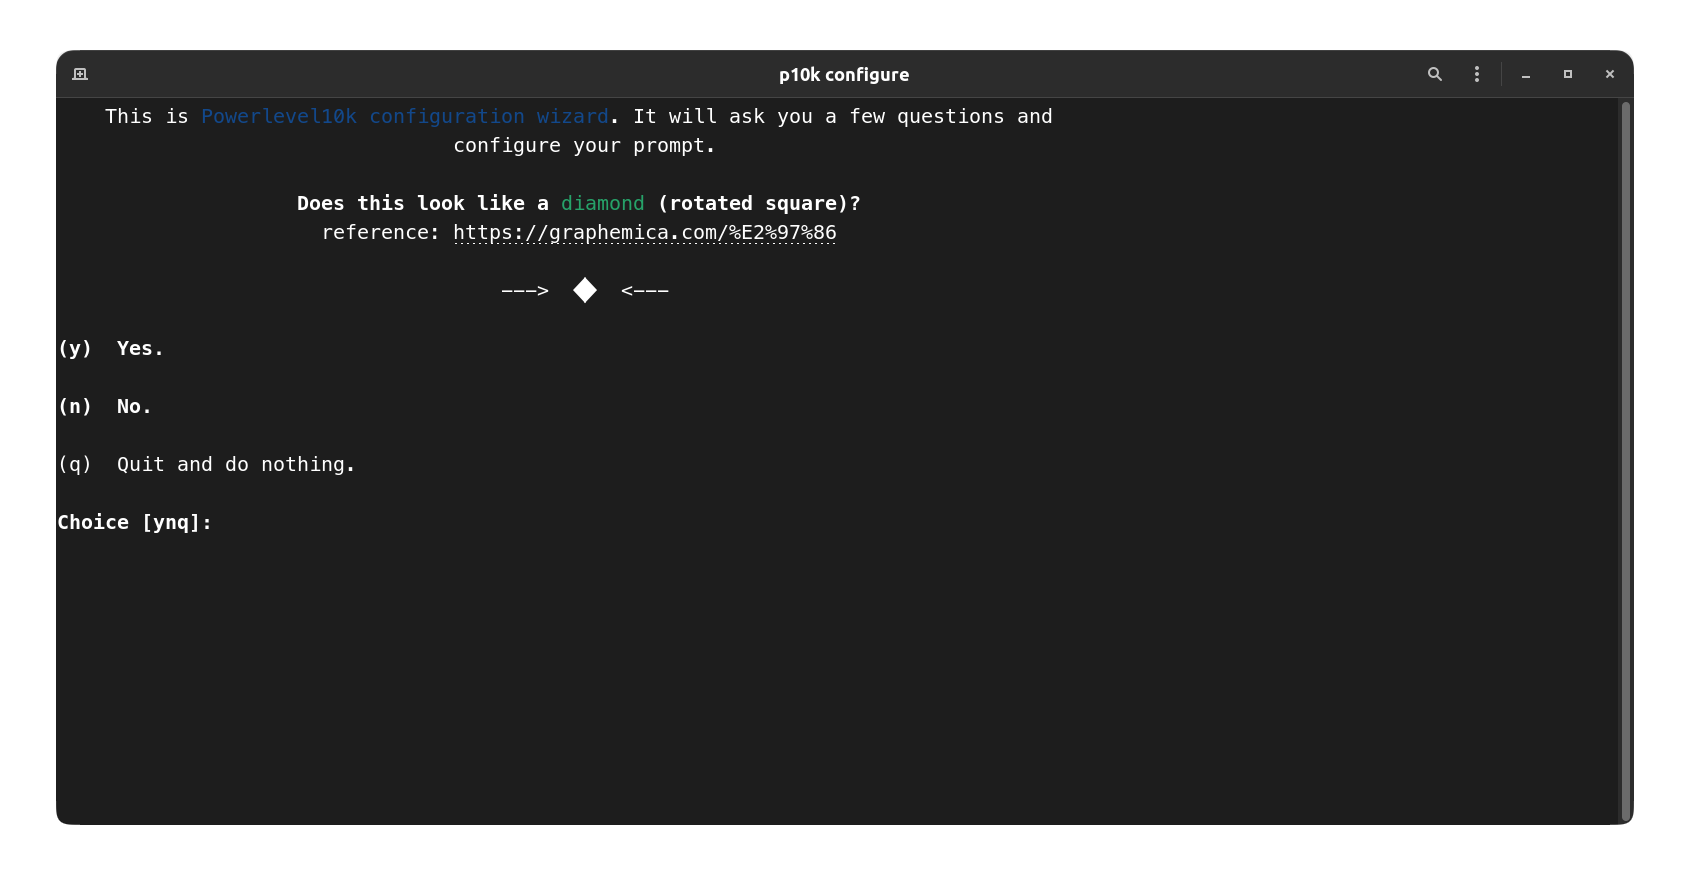
\includegraphics[width=0.8\textwidth]{zsh_p10k_configure.png}}{%
        \fbox{\parbox[c][6em][c]{0.8\textwidth}{\centering 占位图：p10k 配置向导界面（待补充截图）}}}
    \caption{p10k 配置向导}
    \label{fig:p10k_configure}
\end{figure}

\begin{note}
p10k 提示符里的图标（文件夹、git 分支符号等）依赖 Nerd Font 字体，推荐按 p10k 文档安装 MesloLGS NF，并在终端设置中把字体改为它，否则图标会显示为方块或问号。字体下载地址：\url{https://github.com/romkatv/powerlevel10k#fonts}
\end{note}

\textbf{推荐插件}

zsh 的插件生态是它相比 bash 的一大优势，最常用的两个：

\begin{itemize}
\item zsh-autosuggestions：根据历史命令给出灰色补全建议，按方向键右键采纳；
\item zsh-syntax-highlighting：命令输入时实时高亮，命令拼错时显示为红色。
\end{itemize}

\begin{example}
安装这两个插件并在 \textasciitilde/.zshrc 中启用：
\begin{tbash}
git clone https://github.com/zsh-users/zsh-autosuggestions ~/.oh-my-zsh/custom/plugins/zsh-autosuggestions
git clone https://github.com/zsh-users/zsh-syntax-highlighting ~/.oh-my-zsh/custom/plugins/zsh-syntax-highlighting
\end{tbash}
然后修改 \textasciitilde/.zshrc 中的插件行：
\begin{tbash}
plugins=(git zsh-autosuggestions zsh-syntax-highlighting)
\end{tbash}
\end{example}

% TODO(占位图)：配置完成的终端效果图（含 p10k 提示符、自动建议、语法高亮），保存为 images/zsh_p10k_effect.png
\begin{figure}[H]
    \centering
    \IfFileExists{images/zsh_p10k_effect.png}{%
        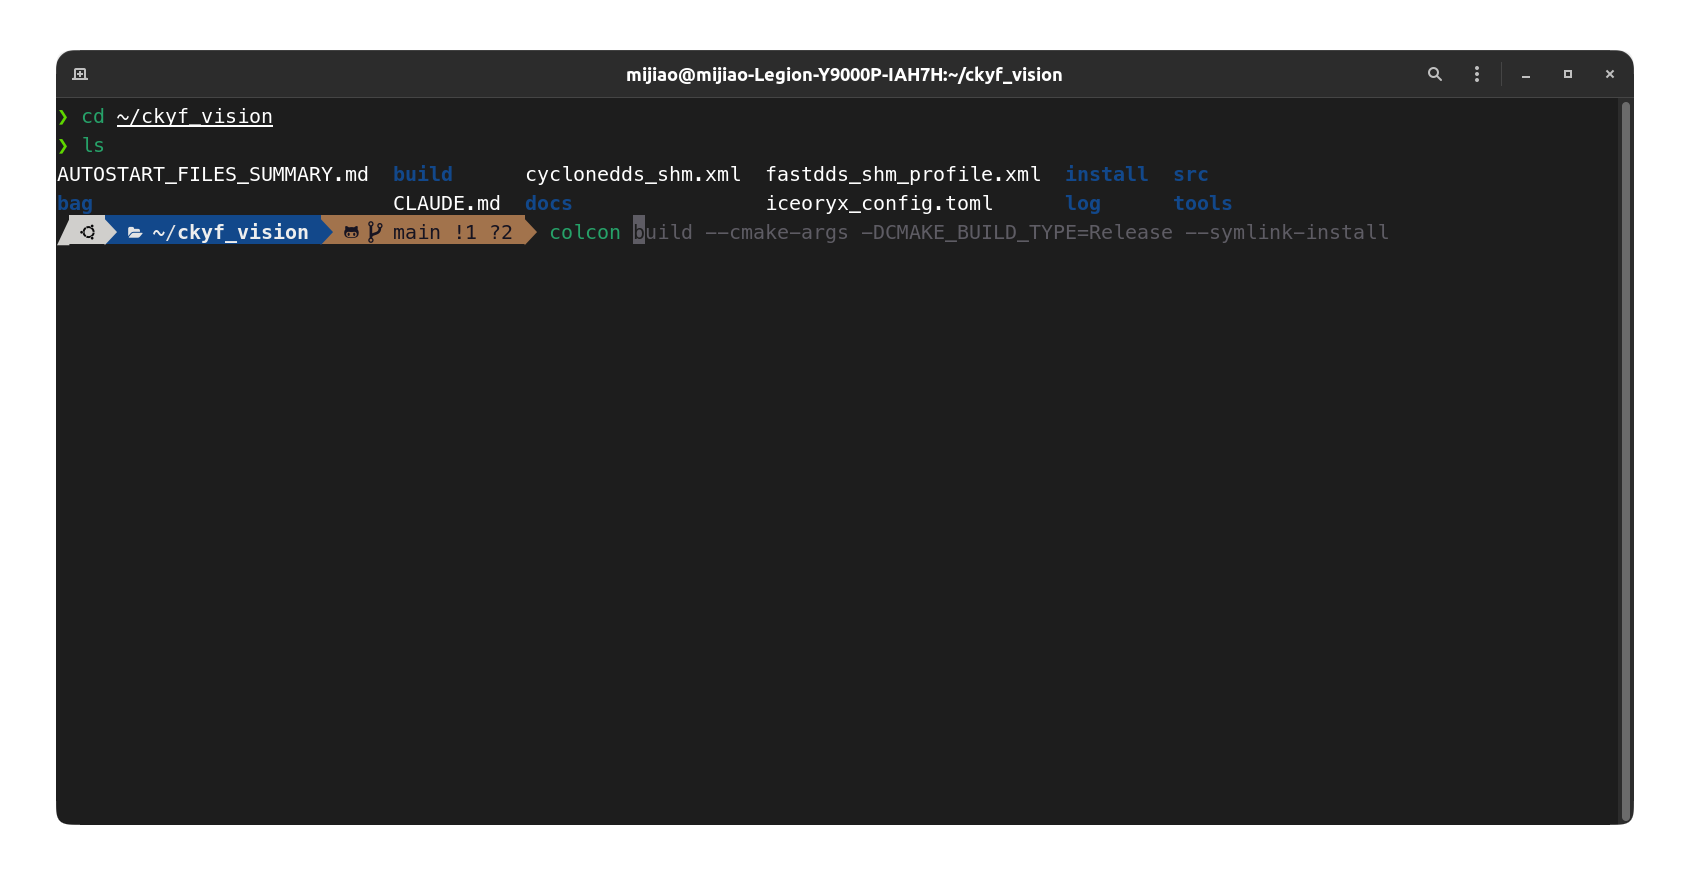
\includegraphics[width=0.8\textwidth]{zsh_p10k_effect.png}}{%
        \fbox{\parbox[c][6em][c]{0.8\textwidth}{\centering 占位图：美化后的终端效果（待补充截图）}}}
    \caption{配置完成后的终端效果}
    \label{fig:zsh_effect}
\end{figure}

\textbf{与 bash 的不同}

换用 zsh 后，日常使用的大部分命令完全一样，但有一些区别需要知道：

\begin{conclusion}
zsh 与 bash 的主要区别：

\begin{center}
\begin{tabular}{ccc}
\toprule[1.5pt]
对比项 & bash & zsh\\
\midrule[1pt]
配置文件 & \textasciitilde/.bashrc & \textasciitilde/.zshrc\\
通配符无匹配时 & 原样保留（如 \texttt{*.txt}） & 报错 no matches found\\
数组下标 & 从 0 开始 & 从 1 开始\\
Tab 补全 & 基础补全 & 支持命令参数、选项的智能补全\\
\bottomrule[1.5pt]
\end{tabular}
\end{center}

两者脚本语法大部分兼容；带 \texttt{\#!/bin/bash} 行首的脚本仍由 bash 执行，更换交互式 shell 不影响已有脚本的运行。
\end{conclusion}

\begin{note}
\textasciitilde/.bashrc 中的内容不会自动迁移到 \textasciitilde/.zshrc——尤其是 source 类的环境配置行（后续卷二安装 ROS2 时会向 \textasciitilde/.bashrc 写入 source 命令）。换用 zsh 后记得手动把这些行加到 \textasciitilde/.zshrc 里，否则会出现"昨天还能编译，今天找不到命令"的灵异事件。
\end{note}

\begin{exercise}
完成 zsh、Oh My Zsh、p10k 的安装与主题配置，启用 autosuggestions 插件，并把原来 \textasciitilde/.bashrc 中自己添加的别名迁移到 \textasciitilde/.zshrc。
\end{exercise}

